\documentclass[oneside,a4paper,14pt]{extarticle}
\usepackage[a4paper,letterpaper,top=20mm,bottom=20mm,left=20mm,right=10mm]{geometry}
\usepackage[russian]{babel}
\usepackage{indentfirst}
\usepackage{graphicx}
\usepackage{caption}
\usepackage{titlesec}
\usepackage{minted, fancyvrb}
\usepackage{hyperref}
\usepackage{enumitem}

\setminted{style = rainbow_dash, fontsize = \small}

\titleformat{\section}{\normalsize\bfseries}{\thesection}{1em}{}
\titleformat{\subsection}{\normalsize\bfseries}{\thesubsection}{1em}{}
\titleformat{\subsubsection}{\normalsize\bfseries}{\thesubsubsection}{1em}{}

\renewcommand\baselinestretch{1.33}
\setlength{\parindent}{1.25cm}

\setlist[enumerate]{
  left=\parindent,
  label=\arabic*.,
  itemsep=0pt,
  topsep=5pt,
  partopsep=0pt,
  parsep=0pt
}

\setlist[itemize]{
  left=\parindent,
  itemsep=0pt,
  topsep=5pt,
  partopsep=0pt,
  parsep=0pt
}

\hypersetup{
  colorlinks=true,
  linkcolor=black,
  urlcolor=blue,
  pdfborder={0 0 0},
  pdftitle={Веб-конструктор Tilda},
  pdfauthor={Черкасов А.А.}
}

\begin{document}

\newpage
\thispagestyle{empty}
\begin{center}
  МИНИСТЕРСТВО НАУКИ И ВЫСШЕГО ОБРАЗОВАНИЯ РОССИЙСКОЙ ФЕДЕРАЦИИ\\
  ФЕДЕРАЛЬНОЕ ГОСУДАРСТВЕННОЕ БЮДЖЕТНОЕ ОБРАЗОВАТЕЛЬНОЕ УЧРЕЖДЕНИЕ ВЫСШЕГО ОБРАЗОВАНИЯ\\
  «ВЯТСКИЙ ГОСУДАРСТВЕННЫЙ УНИВЕРСИТЕТ»\\
  Институт математики и информационных систем\\
  Факультет автоматики и вычислительной техники\\
  Кафедра электронных вычислительных машин
\end{center}
\vspace{10mm}

\hfill
\begin{tabular}{l}
  \footnotesize Дата сдачи на проверку:                                          \\
  \footnotesize <<\rule[-1mm]{5mm}{0.10mm}\/>>\rule[-1mm]{20mm}{0.10mm}\ 2025 г. \\
  \footnotesize Проверено:                                                       \\
  \footnotesize <<\rule[-1mm]{5mm}{0.10mm}\/>>\rule[-1mm]{20mm}{0.10mm}\ 2025 г. \\
\end{tabular}
\vfill

\begin{center}
  Разработка веб-сайта с использованием конструктора Tilda.\\
  Отчёт по лабораторной работе №1\\
  по дисциплине\\
  «Технологии Программирования»
\end{center}

\vspace{25mm}

\noindent
\begin{tabular}{ll}
  Разработал студент гр. ИВТб-2301-05-00 & \hspace{18mm}\rule[-1mm]{30mm}{0.10mm}\,/Черкасов А. А./ \\
                                         & \hspace{25.5mm}\footnotesize(подпись)                    \\
  Преподаватель                          & \hspace{18mm}\rule[-1mm]{30mm}{0.10mm}\,/Пащенко Д. Э./  \\
                                         & \hspace{25.5mm}\footnotesize(подпись)                    \\
\end{tabular}

\vfill
\begin{center}
  Киров\\
  2025
\end{center}

\newpage
\section*{Цель лабораторной работы}

Цель: Приобрести практические навыки создания и публикации веб-сайта с использованием конструктора Tilda.

\section*{Задание}

\begin{enumerate}
  \item Согласовать тему создаваемого сайта с преподавателем и внести её в таблицу
  \item Разработать сайт по приложенным методическим материалам
\end{enumerate}

\section*{Решение}

\textbf{Ссылка на опубликованный проект:} \url{https://project19451366.tilda.ws/}

Тема созданного сайта - сайт про милых котиков и других животных. Согласно заданию на сайте были созданы 3 веб-страницы, которые содержали в себе: главную страницу, страницу с галереей фотографий котиков и страницу с собачками.

Для каждой страницы, в качестве стандартного шаблона используются следующие блоки: шапка с навигацией по сайту, подвал с дублирующей навигацией и копирайтом.

На главной странице используются блоки:
\begin{itemize}
  \item[--] Обложка с заголовком <<Милые и смешные>>, подзаголовком и фоновым изображением с котиками
  \item[--] Блок навигации с переходом на страницы котиков и собачек
  \item[--] Форма для предложений добавления животных с текстовым полем и кнопкой <<Отправить>>
\end{itemize}

\begin{figure}[H]
  \centering
  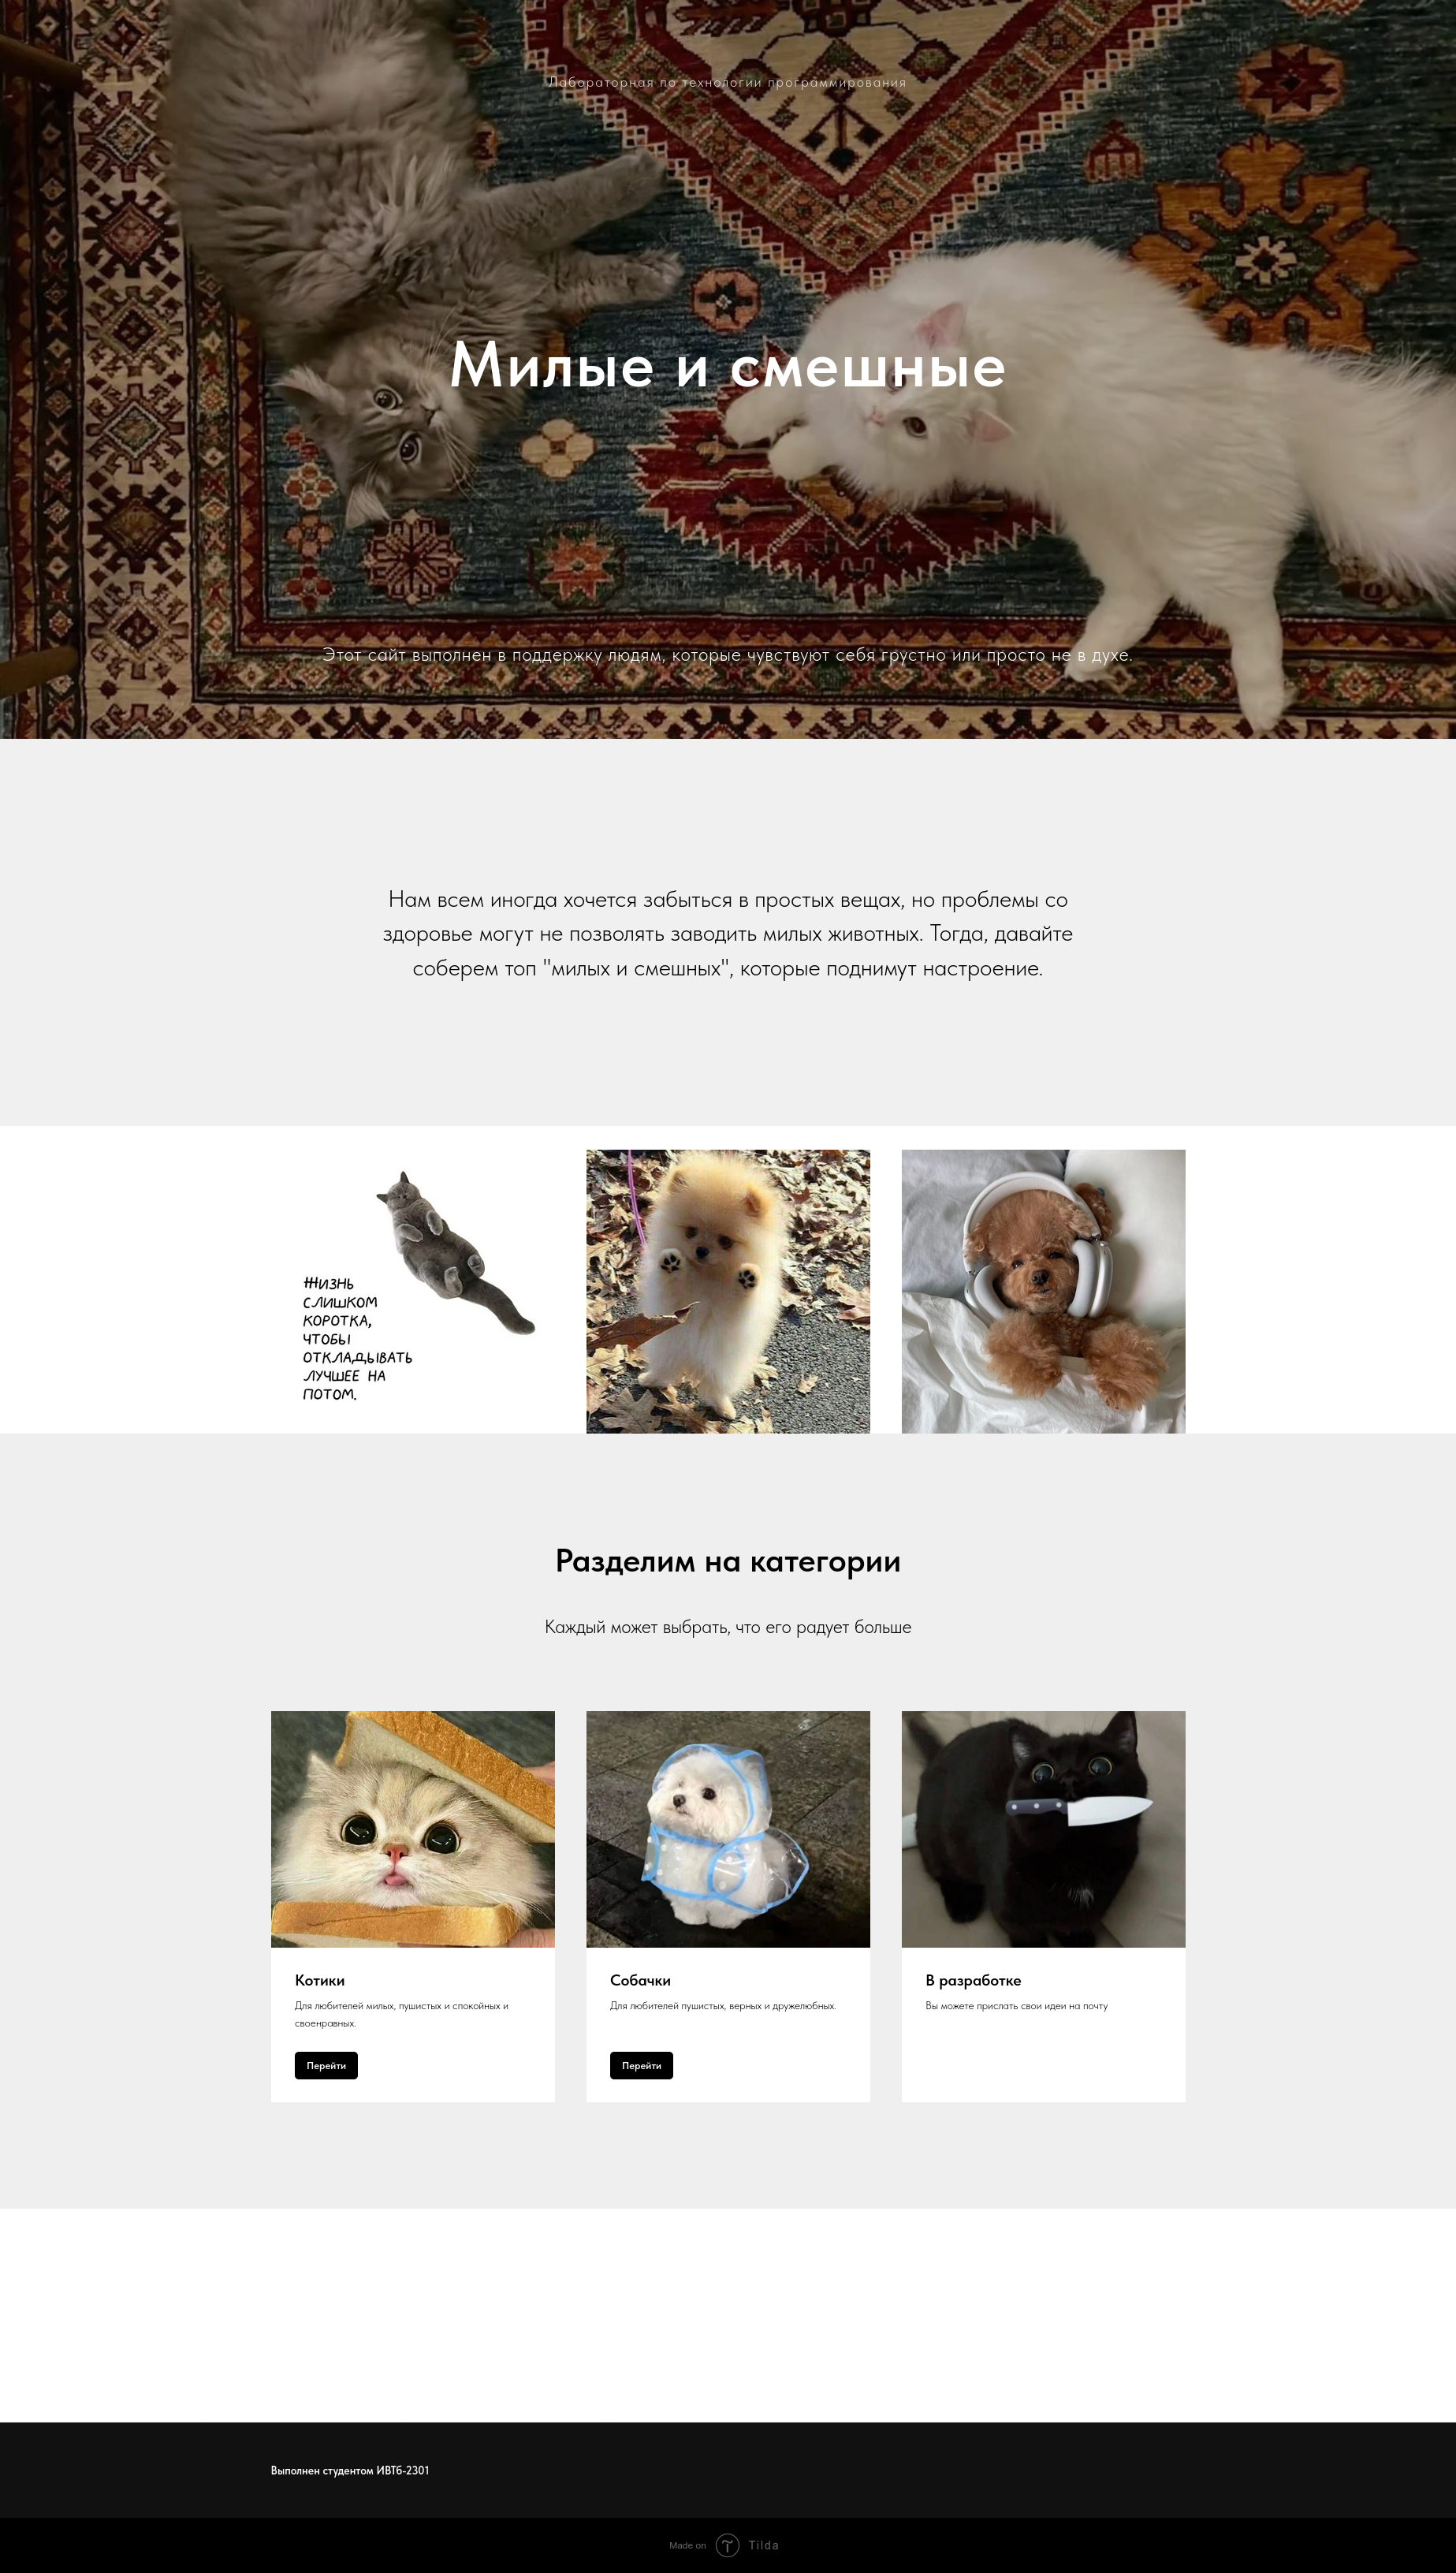
\includegraphics[height=0.95\textheight]{pics/full_main_page.png}
  \caption*{Рисунок 1 --- Главная страница сайта}
\end{figure}

На странице с галереей фотографий котиков используются блоки:
\begin{itemize}
  \item[--] Карточка <<Котики>> с изображением котика в сэндвиче и описанием: <<Для любителей милых, пушистых и спокойных и своенравных>>
  \item[--] Кнопка <<Перейти>> для перехода к галерее
\end{itemize}

На странице с собачками используются блоки:
\begin{itemize}
  \item[--] Карточка <<Собачки>> с изображением собачки в голубом костюмчике и описанием: <<Для любителей пушистых, верных и дружелюбных>>
  \item[--] Кнопка <<Перейти>> для перехода к галерее
\end{itemize}

\begin{figure}[H]
  \centering
  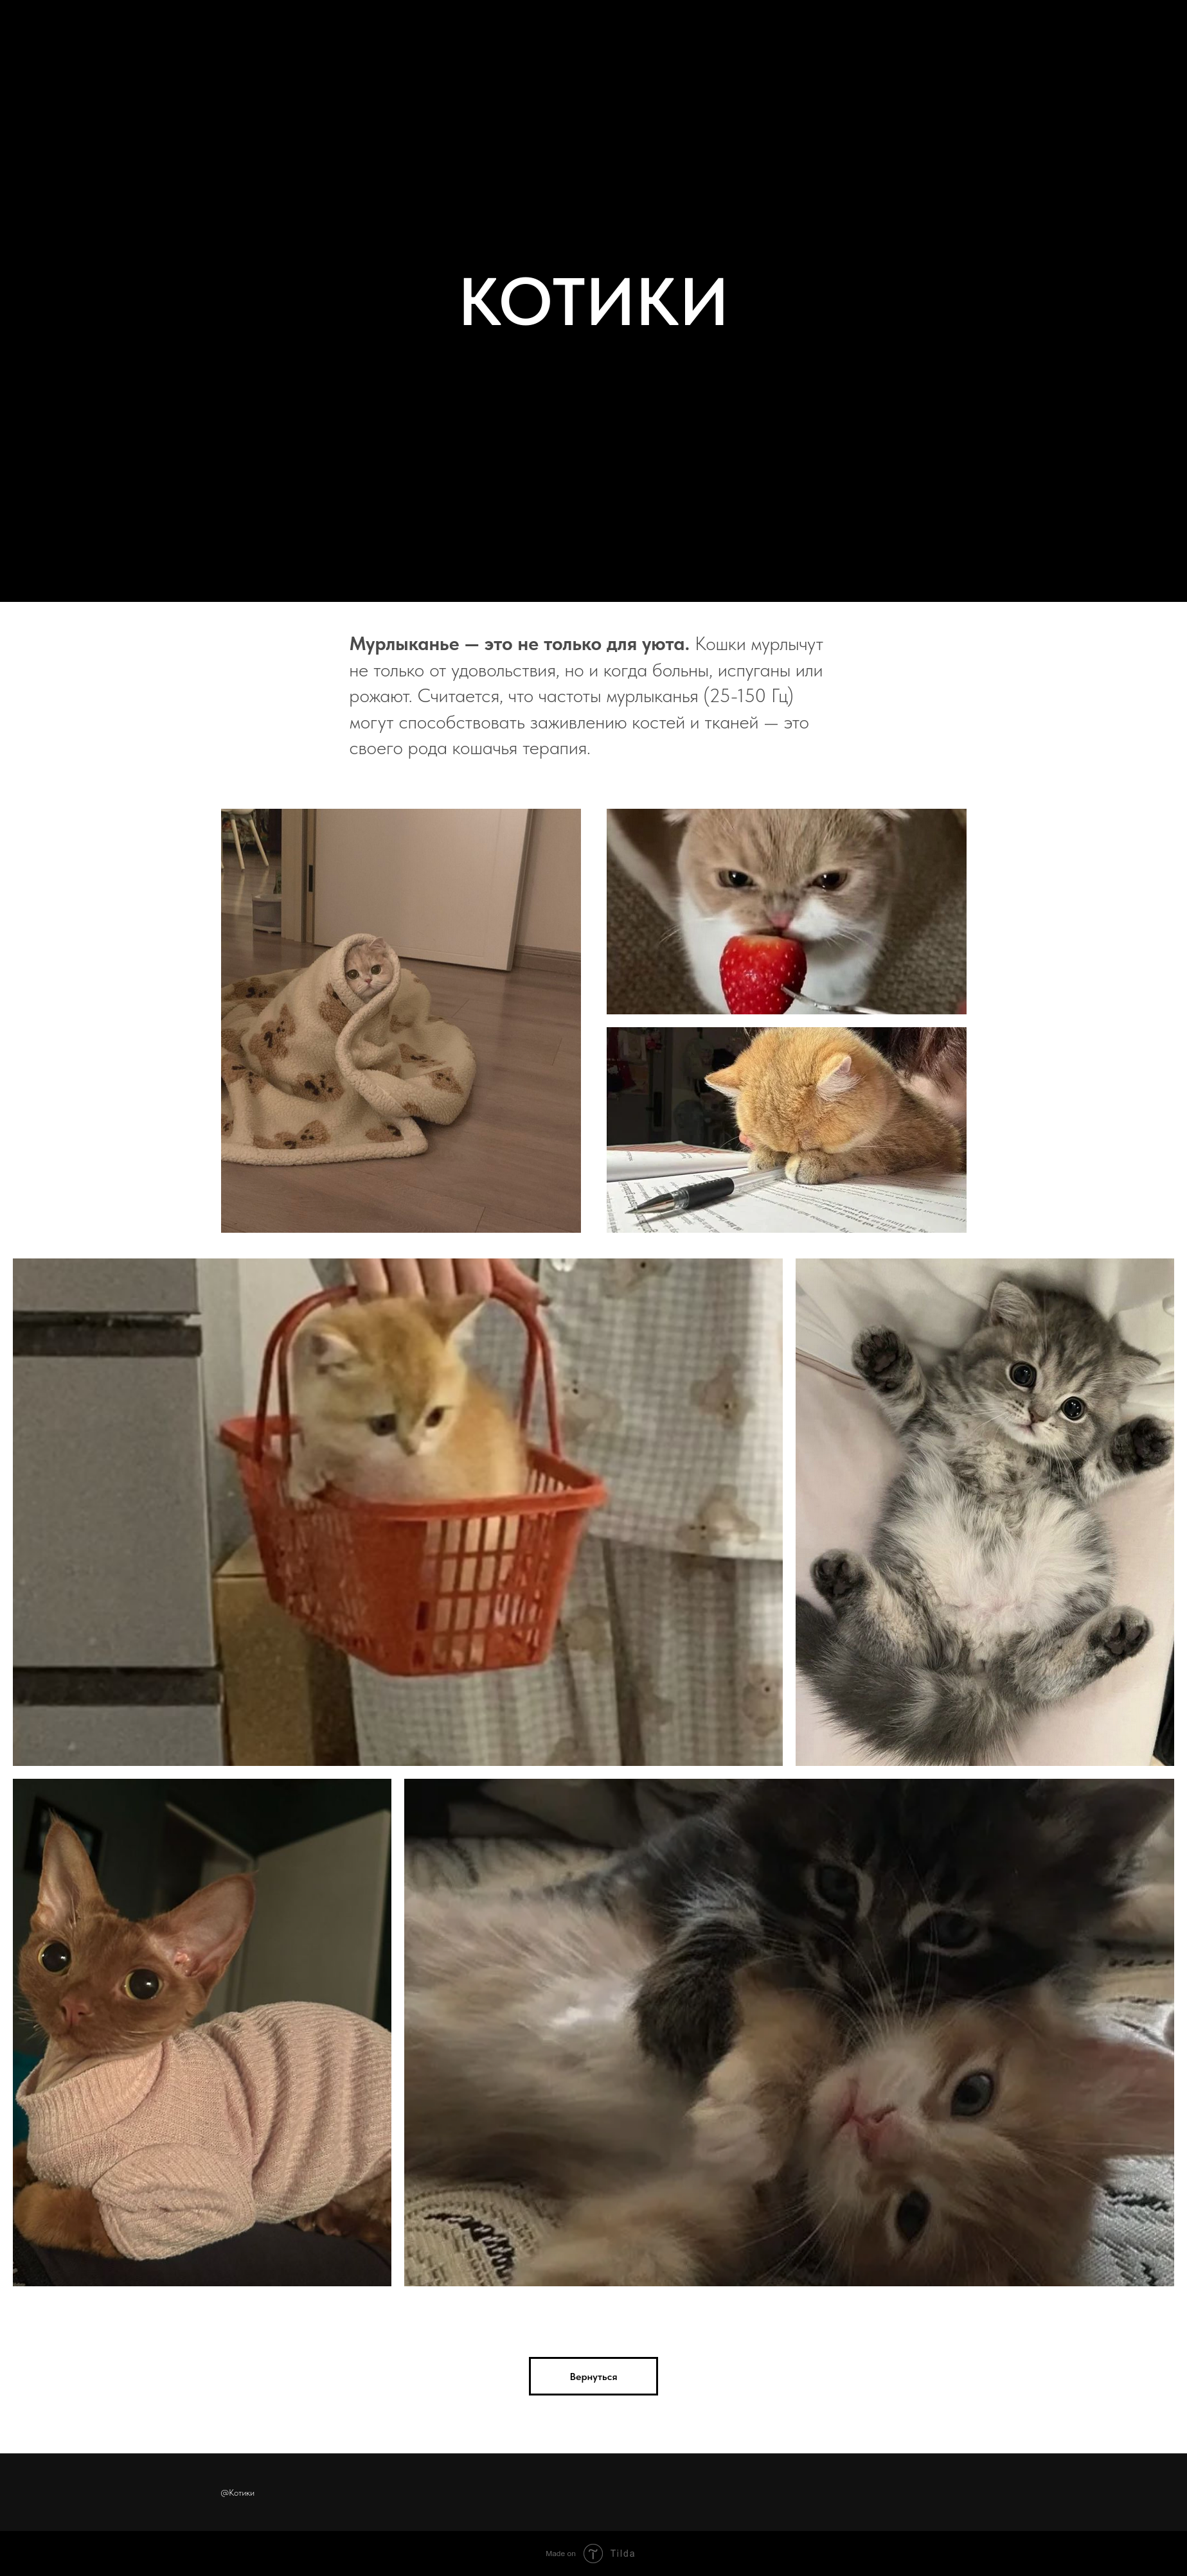
\includegraphics[height=0.95\textheight]{pics/full_cats.png}
  \caption*{Рисунок 2 --- Страница с галереей котиков}
\end{figure}

Также на страницах присутствует карточка <<В разработке>> с изображением черного котика с ножом, предлагающая пользователям присылать свои идеи по почте.

При отправке формы предложений данные отправляются в Google таблицу для дальнейшей обработки.

\begin{figure}[H]
  \centering
  \includegraphics[width=0.8\textwidth]{pics/google_sheets.png}
  \caption*{Рисунок 3 --- Интеграция с Google Таблицами}
\end{figure}

\newpage
\section*{Вывод}

В ходе выполнения лабораторной работы был разработан веб-сайт с использованием конструктора Tilda на тему милых животных.

Была изучена структура веб-проекта на платформе Tilda, освоены основные блоки конструктора: обложки, карточки товаров/услуг, формы обратной связи, навигационные элементы.

Были выполнены все требования задания: создано три веб-страницы с единым стилем оформления, реализована навигация между страницами, добавлена форма для сбора обратной связи с интеграцией в Google таблицы.

Работа позволила приобрести практические навыки работы с современными конструкторами сайтов и понять принципы создания адаптивных веб-страниц без программирования.


\end{document}
